% 10:30
\renewcommand{\konferenztag}{\freitag}
\newsmalltimeslot{09:30}
\abstractNeun{Christoph Hormann}%
{Freie Satellitenbilder -- ein Überblick}%
{Wie man sich frei und neutral ein Bild der Erde machen kann}%
{Bei freien Geodaten auf der FOSSGIS -- da denkt man meist an OpenStreetMap oder andere
kartographische Daten. Dieser Vortrag widmet sich hingegen mal dem Thema der freien Satellitenbilder
und gibt einen grundsätzlichen Überblick darüber, was es in diesem Bereich an freien Daten derzeit
gibt und wie man diese praktisch nutzen kann.}


%2017-03-24 10:30:00
\abstractDreizehn{Daniel J H}%
{Open Source Routing Machine}%
{}
%{Die Open Source Routing Machine (OSRM) ist eine High-Performance-Routingengine und primär für
%OpenStreetMap Daten ausgelegt.}
{Die Open Source Routing Machine (OSRM) ist eine High-Performance-Routing-Engine und primär für
  OSM-Daten ausgelegt. Dieser Vortrag stellt OSRM inklusive Ökosystem vor. Weiterhin
  zeigen wir auf, an welchen Verbesserungen wir im letzten Jahr gearbeitet haben. Wir erklären wie
  OSRM genutzt werden kann, um GPS-Traces auf das Straßennetz zu snappen, wie wir OpenStreetMap
  nutzen, um zum Beispiel Spuren verwenden zu können, und wie Echtzeit Verkehrsdaten eingebunden
werden können.}

\newtimeslot{10:00}
\abstractNeun{Christian Strobl}%
{Freie Fernerkundungsdaten für alle – das Copernicus-Programm der EU}%
{Freie Sentinel-Daten mit freier Software}%
{Von den Sentinel-Missionen der EU haben viele GIS"=Anwender bereits gehört oder gelesen. Tatsächlich
mit den jetzt schon verfügbaren Daten der Sentinel-1 (S-1), Sentinel"=2 (S-2) und Sentinel-3 (S-3)
Daten gearbeitet haben aber bisher nur wenige Fernerkundler. Dieser Vortrag gibt einen Überblick
über alle Sentinel-Missionen sowie möglicher Anwendungsfälle. Dazu werden Download, Eingabe,
Ansicht, Prozessierung und Analyse von S-1- und S-2-Daten mit freier Software aufgezeigt und
beispielhaft vorgeführt. Abgerundet wird der Vortrag durch einen allgemeinen Überblick über das
Copenicus-Programm.}



%2017-03-24 11:00:00
\abstractDreizehn{Michael Zilske}%
{Öffentlicher Verkehr in\newline GraphHopper}%
{}%
{Wir entwickeln ÖV-Funktionen für den OSM"=Router GraphHopper. In diesem Vortrag möchten
wir zeigen, was damit schon möglich ist, alles basierend auf OSM-Daten für das Straßennetz und
GTFS-Daten für das ÖV-Angebot.}

\newtimeslot{11:00}
\abstractNeun{Stefan Küspert}%
{Steigerung der Akzeptanz\newline räumlicher Planung durch freiwillig gesammelte Geodaten}%
{}%
{Hatten Sie schon einmal das Gefühl, dass die Meinung der Bürger zu einem Projekt Ihrer Gemeinde
nicht gehört wird, regionales Wissen nicht wertgeschätzt wird, oder Informationen nicht transparent
und verständlich dargestellt werden? Dieser Vortrag präsentiert Ergebnisse aus dem
BMBF-Forschungsprojekt PUBinPLAN, welches OSM, geobasiertes Crowdsourcing und Augmented
Reality verwendet, um mehr Beteiligung in räumlichen Planungsprozessen zu erreichen. }

\abstractDreizehn{Jochen Topf}%
{OSM-Daten verarbeiten auf der \mbox{Kommandozeile} mit Osmium}%
{}%
{Aufbauend auf der schnellen und flexiblen Osmium-C++-Bibliothek hat sich das
Osmium-Kommandozeilentool zu einem nützlichen Helferlein entwickelt. Wer Osmium in seiner
Werkzeugkiste hat, kann neue Wege gehen beim Verarbeiten von OSM-Daten. Mit Beispielen aus der
Praxis will ich zeigen, was das Tool kann, und wo und wie man es einsetzt.}

\newtimeslot{11:30}
\abstractNeun{Johannes Kröger}%
{GeoPackages der freien Hamburger Geodaten}%
{}%
{Im Hamburger Transparenzportal finden sich unterschiedlichste Geodaten, beispielsweise georeferenzierte
  Hausnummern, Gebäudemodelle, das Straßenbaumkataster, Teile von ALKIS, Höhenmodelle, Luftbilder und
  Verkehrs- und Umweltdaten.

Viele der Daten liegen in "`rohen"' oder speziellen Formaten vor, was ihre Verwendung von Laien
erschwert. Mit einer automatisierten und reproduzierbaren Umwandlung in standardkonforme GeoPackages
können die Geodaten einfachstmöglich in QGIS u.ä. verwendet werden.

Vorgestellt werden Ansätze, Probleme, Tipps und sowie die bis zur FOSSGIS fertig aufbereiteten
Datensätze.}

\abstractDreizehn{Pascal Neis}%
{Vandalismus im OSM-Projekt}%
{Stand heute. Und morgen?}%
{
Der Zulauf zum OpenStreetMap-Projekt ist ungebrochen. Leider bringt diese stets
steigende Anzahl von aktiven Mitgliedern auch Nachteile mit sich. In den
letzten Jahren gab es immer wieder Fälle, bei denen bewusst oder unbewusst
vorhandene OSM-Objekte aus der Datenbank des Projektes gelöscht wurden.}

\newtimeslot{12:00}
\abstractNeun{Felix Kunde}%
{Mit Deep Learning raum-zeitliche Muster erkennen und voraussagen}%
{}%
{Die Begriffe Deep Learning und künstliche Intelligenz sind gerade in aller Munde~--
auch in der GIS-Welt. Was ist dran an dem Hype? In dem Vortrag sollen einige
freie Projekte vorgestellt werden, in denen Deep-Learning-Methoden auf Geodaten
angewandt werden.}

\abstractDreizehn{Alexander Matheisen}%
{Zusammenführung und Vereinheitlichung von Eisenbahn-Streckennetzdaten}%
{}%
{Bei der Erstellung von grenzüberschreitenden Karten zur Information von Bahnreisenden stellen die
zu Grunde liegenden Daten eine besondere Herausforderung dar. Verschiedene Bahngesellschaften bieten
mittlerweile im Rahmen von Open-Data-Initiativen Datensätze zu ihren Streckennetzen an. Daneben
stellt auch OpenStreetMap entsprechende Daten bereit. Doch alle diese Datensätze liegen in
unterschiedlichen Formaten und Datenmodellen vor und bilden jeweils nur begrenzte Gebiete ab. Dies
erschwert die weitere Arbeit mit diesen Daten und erfordert eine vorherige Zusammenführung und
Vereinheitlichung der Datensätze.}

\newtimeslot{13:15}
\abstractNeun{Bastian Drees}%
{OSGeo-Konferenzaufzeichnungen im TIB AV-Portal\vspace{0.2\baselineskip}}%
{Wissenschaftliche Ressourcen dauerhaft bewahren und innovativ nutzen.}%
{Mit dem AV-Portal (av.tib.eu) stellt die Technische Informationsbibliothek (TIB) eine
nutzerorientierte Plattform zur Verfügung, die OSGeo-Konferenzaufzeichnungen dauerhaft verfügbar,
durchsuchbar und zitierfähig bewahrt. Seit 2016 ist die Howto-Anleitung für den AV-Portal-Ingest
Teil des offiziellen OSGeo-Konferenzhandbuchs. Innovative  Videoanalysen ermöglichen die Suche im
gesprochenen und geschriebenen Text der Videos. Die Verbindung eines DOI mit einem Media Fragment
Identifier gewährleistet eine sekundengenaue Zitierfähigkeit der Materialien.}

\sponsorenboxA{208-sourcepole.png}{0.4\textwidth}{3}{%
\textbf{Bronzesponsor, Aussteller}\\
Sourcepole bietet diverse Dienst\-leistungen im Bereich Open-Source-GIS an,
unter anderem QGIS Cloud. QGIS Cloud ist ideal für Unternehmen,
welche die Vorteile einer verteilten Geodateninfrastruktur nutzen wollen, ohne selber
Datenbank, Webserver und Kartenserver zu betreiben.}


\newsmalltimeslot{13:30}
\abstractNeun{Peter Barth}%
{OSM-Ehrenamt}%
{Freiwillige Arbeit jenseits des Daten-Mappings}%
{Das OpenStreetMap-Projekt ist eine große weltweite Community aus
Freiwilligen, die aber nicht nur aus Mappern besteht sondern allgemein
eine Vielzahl weiterer Aufgaben erledigen, um das
Projekt am Laufen zu halten. Der Vortrag wirft ein Licht auf die
Tätigkeits- und Aufgabenbereiche der verschiedenen Arbeitsgruppen,
versucht deren bisherige Leistungen hervorzuheben und soll zudem
aufzeigen, wo und wie man sich beteiligen kann.}

\newsmalltimeslot{16:00}
\abstractDreizehn{}%
{Qualitätsoffensive OSM}%
{Gemeinsamer Mappingevent zum Erlernen und Vertiefen der OpenStreetMap-Kenntnisse}%
{Nach einer kurzen Einführung und Absprache um 16:00 Uhr sammeln die Teilnehmer in Gruppen
mit unterschiedlichen Themenschwerpunkten Daten in der Passauer Innenstadt. Im Anschluss
werden die gesammelten Daten dann gemeinsam in die Karte eingepflegt.
Das Spektrum möglicher Themen reicht, je nach Interesse und Erfahrung, vom Eintragen von
Ladengeschäften bis zum 3D- und Indoor-Mapping. Das Mappingevent ist auch für Anfänger geeignet.}

\sponsorenboxA{205-optitool}{0.5\textwidth}{3}{%
  \textbf{Bronzesponsor}\\
  OPTITOOL ist eine führende Softwarelösung für Tourenplanung und
  Tourenoptimierung. Mit Hilfe von OPTITOOL ermitteln Sie den kostengünstigsten
  Tourplan, der spezielle Branchengegebenheiten und alle für Sie wichtigen
  Restriktionen berücksichtigt.
}

\vfill
\sponsorenboxA{204_geofabrik}{0.53\textwidth}{3}{%
  \textbf{Bronzesponsor}\\
  Die Geofabrik GmbH ist ein OSM"=Expertenbüro in Karlsruhe. 
  Seit 2007 extrahiert, filtert und verarbeitet die Geofabrik für Sie 
  freie Geodaten, erzeugt Shapefiles, Kartenbilder, Kacheln oder 
  komplette Web-Kartenanwendungen. Die Geofabrik ist spezialisiert 
  auf Dienstleistungen rund um OpenStreetMap, wie Beratung, Datenexport, 
  Server-Setup und Software-Entwicklung.
}

\vfill
\sponsorenboxA{301_oreilly}{0.5\textwidth}{5}{%
\textbf{Mediapartner}\\
O'Reilly-Bücher vermitteln praxis\-orientiertes Know-how aus den Bereichen IT
(Programmierung, Administration), Business, Gründen und Social Media sowie
Elektronik und DIY. Deutsche O'Reilly-Bücher werden vom dpunkt.verlag in
Heidelberg publiziert.}


\sponsorenboxA{206-terrestris}{0.27\textwidth}{3}{%
\textbf{Bronzesponsor, Aussteller}\\
terrestris bietet Dienstleistungen und Produkte mit Open-Source-Software an und 
ist dabei insbesondere auf Geodateninfrastrukturen, webbasierte Informationssysteme und WebMapping-Anwendungen fokussiert, 
die neben 2D- auch 3D-Daten enthalten und auch für mobile Endgeräte optimiert sind.
%Wir orientieren uns dabei an den Anforderungen unserer Kunden und realisieren auf 
%den jeweiligen Bedarf zugeschnittene Lösungen.
%Neben der Anwendungsentwicklung können unsere Kunden Support und Schulungen für 
%verschiedene Open-Source-Softwaretools, z.\,B. PostgreSQL/PostGIS, UMN Mapserver, 
%GeoServer, SHOGun, OpenLayers, GeoExt, ExtJS und QGIS, erhalten \dots
}

\vfill
\sponsorenboxA{602-osgeolive}{0.55\textwidth}{3}{%
\textbf{OSGeo-Live}\\
Die OSGeo-Live ist eine bootfähige DVD, USB-Stick oder eine virtuelle Maschine auf Lubuntu-Basis und
bietet Ihnen die Möglichkeit, freie und Open-Source-Software in Verbindung mit
Geodaten auszuprobieren, ohne aufwendige Installationen durchführen zu müssen. Das
Projekt wird von der OSGeo Foundation und vielen weiteren Aktiven getragen.}


\newpage
% neuer Layer für Geländeplan
\DeclareNewLayer[background, oddorevenpage,  width=125mm,%
height=169mm, contents={%
  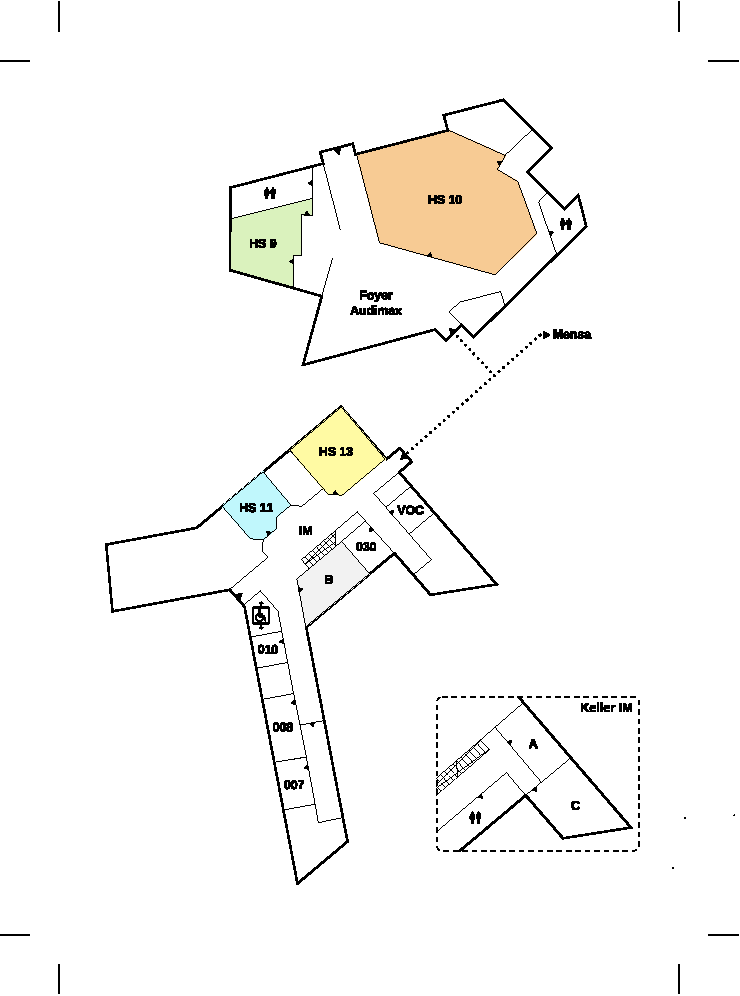
\includegraphics{wallpaper/raumplan-a6.pdf}%
}]{raumplana6}
\newpairofpagestyles[scrheadings]{raumplan}{}
\AddLayersAtBeginOfPageStyle{raumplan}{raumplana6}
\pagestyle{raumplan}
\null
\label{raumplan-page}
